\chapter{%
ROSデジタルツインシステムの検証}

前章では,開発したROSデジタルツインシステムについて説明した.
本章では,システムを検証するための実験について述べる.第3.1章で実験方法と実験環境について説明し,第3.2章でデジタルツインの検証方法を述べ,第3.3章で実験結果を,第3.4章で考察を述べる.

\section{実験方法}
本節では実験方法ついて実験環境と実験手順を述べる.
\subsection{実験環境}
本節では,実験環境について使用機器やそれらの接続方法について述べる.\\
 実験には図3.1.1に示す機器を使用した.PCのOS環境はUbuntu20.04でROS環境はNoeticである.Lite6は電源からパワーアダプタと緊急ボタンを経て給電され,ルーターを介してPCに接続される.
切り紙グリッパー内のDYNAMIXELモータは電源からDXSharingBoardを経て給電され,PCとDYNAMIXELモータの双方向通信のためのUSBシリアルインターフェースであるU2D2を介してPCに接続される.
また,Lite6は机の上の端に設置して2個のクランプによって固定し,Lite6のエンドエフェクタに自作のコネクタを介して切り紙グリッパーを接続している.

\begin{figure}[htbt]
    \centering
     \includegraphics[height=80mm]{expt_environment.eps}
     \caption{実験環境}
     \label{fig:f2}
\end{figure}

\begin{figure}[htbt]
    \centering
     \includegraphics[height=70mm]{expt_connect.eps}
     \caption{使用機器の接続図}
     \label{fig:f2}
\end{figure}

\subsection{実験手順}
前章で述べたように,現状,開発したシステムは物理モデルとデジタルモデルの制御を同時に行うことができない.そのため,まず,物理モデルの実験を行い,その後にデジタルモデルの実験を行う.\\
 物理モデルの実験は,前章で述べた物理モデルの動作前準備にデータ収集のためのrosbagコマンドの実行を加えた手順でノードを正しい順番に立ち上げて行う.その手順について以下で改めて説明する.
まず,roscoreでMasterを立ち上げ,rosbagコマンドを実行してトピックの記録を開始する.次に,Lite6 bring upノードでLite6を起動し,ros\_controlノード,MoveIt\&RVIZノード,Motion plannerノード,Dynamixel workbench controllersノードの順に立ち上げる.
以上の手順が完了したら,Target motionノードを実行してLite6の手先位置制御を行う.このノードでは目標手先座標としてLite6の基準座標系(Base coordinate)から見た値で(0.20750, -0.10000, 0.25875) mを設定する.
最後に,物理モデルの手先が移動して静止したら,切り紙グリッパーを閉じるための位置指令をターミナルからrosservice callコマンドで送信する.この実験では切り紙グリッパーが完全に閉じるために$720^\circ$回転するよう位置指令を出す.\\
 デジタルモデルの実験は前章で述べたデジタルモデルのシミュレーション前準備にデータ収集のためのrosbagコマンドの実行を加えた手順でノードを正しい順番に立ち上げて行う.その手順について以下で改めて説明する.
まず,roscoreでMasterを立ち上げ,rosbagコマンドを実行してトピックの記録を開始する.次に,切り紙グリッパーを開くための位置指令をターミナルからrostopic pubコマンドで送信する.これにより指の初期位置を開いた状態にする.
次に,Gazebo spawnerノードでワールドと切り紙グリッパーを持つLite6のURDFファイルを読み込み,Gazeboにデジタルモデルを表示する.
次に,ros\_controlノード,MoveIt\&RVIZノード,Motion plannerノードの順に立ち上げる.
以上の手順が完了したら,Target motionノードを実行してLite6の手先位置制御を行う.このノードは物理モデルの実験と同様に目標手先座標としてLite6の基準座標系から見た値で(0.2075, -0.1, 0.25875) mを設定する.
最後に,デジタルモデルの手先が移動して静止したら,切り紙グリッパーを閉じるための位置指令をターミナルからrostopic pubコマンドで送信する.



\section{デジタルツインの検証方法}
このROSデジタルツインシステムはロボットアームの手先位置と切り紙グリッパーの指先距離のデジタルツインを目的に開発した.
以下ではそれぞれのデジタルツインシステムがどの程度の精度を持っているのかを定量的に検証する方法を述べる.\\
 まず,ロボットアームの手先位置のデジタルツインシステムの検証方法を述べる.このシステムにおいて入力はTarget motionノードで設定した目標手先座標であり,出力はLite6の物理モデルとデジタルモデルの関節角度である.
このことから,Lite6の基準座標系から手先座標系までの同次変換行列を求め,その行列にTarget motionノードを実行した後のLite6の全ての関節角度を入力することにより実際の手先座標を計算し,目標手先座標と比較して検証を行う.\\
 次に,切り紙グリッパーの指先距離のデジタルツインシステムの検証方法を述べる.切り紙グリッパーの物理モデルでは開閉時のグリッパーの中心から指先までの距離を実測済みである.
デジタルツインの精度を確認するためにはGazebo内のデジタルモデルの開閉時のグリッパーの中心から指先までの距離を測定する必要がある.
そこで,デジタルモデルのFinger1\_jointを関節軸に持つFinger1リンクの先端にジョイントを追加し,切り紙グリッパーを開閉した時のその座標の変化をrosbagコマンドでGazebo/link\_statesトピックの記録から取得することで目的の距離を測定し,実測値と比較して検証を行う.
また,物理モデルとデジタルモデルの制御の実行時間についても評価を行う.

\begin{figure}[htbt]
    \centering
     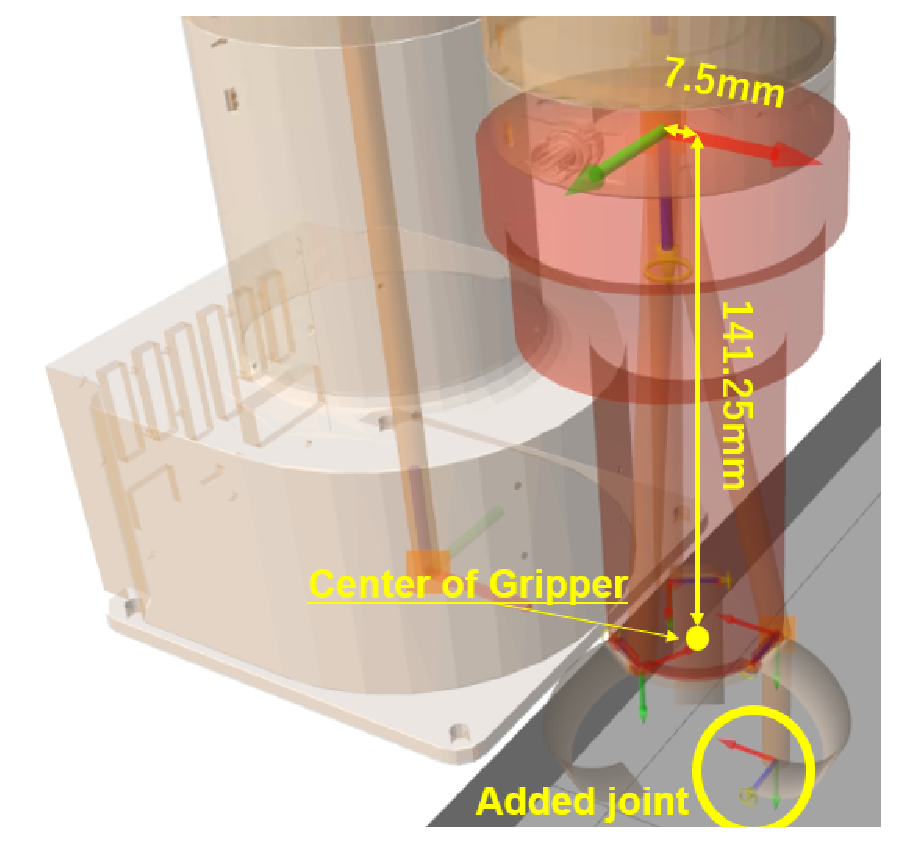
\includegraphics[height=55mm]{measure_joint.eps}
     \caption{切り紙グリッパーの指先距離を測定するためのジョイント}
     \label{fig:f2}
\end{figure}

\section{実験結果}
本節では,物理モデルとデジタルモデルの実験結果について述べる.
\subsection{物理モデルの実験結果}
まず,物理モデルの実験結果を以下に示す.
図3.4から,0sから5sにかけて手先が目標の手先座標に移動していることがわかり,このとき各関節の角度は図3.5に示すように変化した.変化後の各関節の角度を表3.1にまとめる.
また,Lite6の基準座標系から手先座標系までの同次変換行列に表3.1の角度を代入して計算すると実際の手先座標は(0.177674, -0.0850884, 0.268573) mになった.\\
 そして,図3.4から7sから9sにかけて切り紙グリッパーが閉じていることがわかる.このとき切り紙グリッパー内のDYNAIMXELモータの角度は図3.6に示すように変化した.
したがって,到達角度はラジアン値で-12.567であり,約$-720.04^\circ$になった.

\begin{figure}[htbt]
    \centering
     \includegraphics[height=90mm]{realmove.eps}
     \caption{物理モデル実験の結果}
     \label{fig:f2}
\end{figure}

\begin{figure}[htbt]
    \centering
     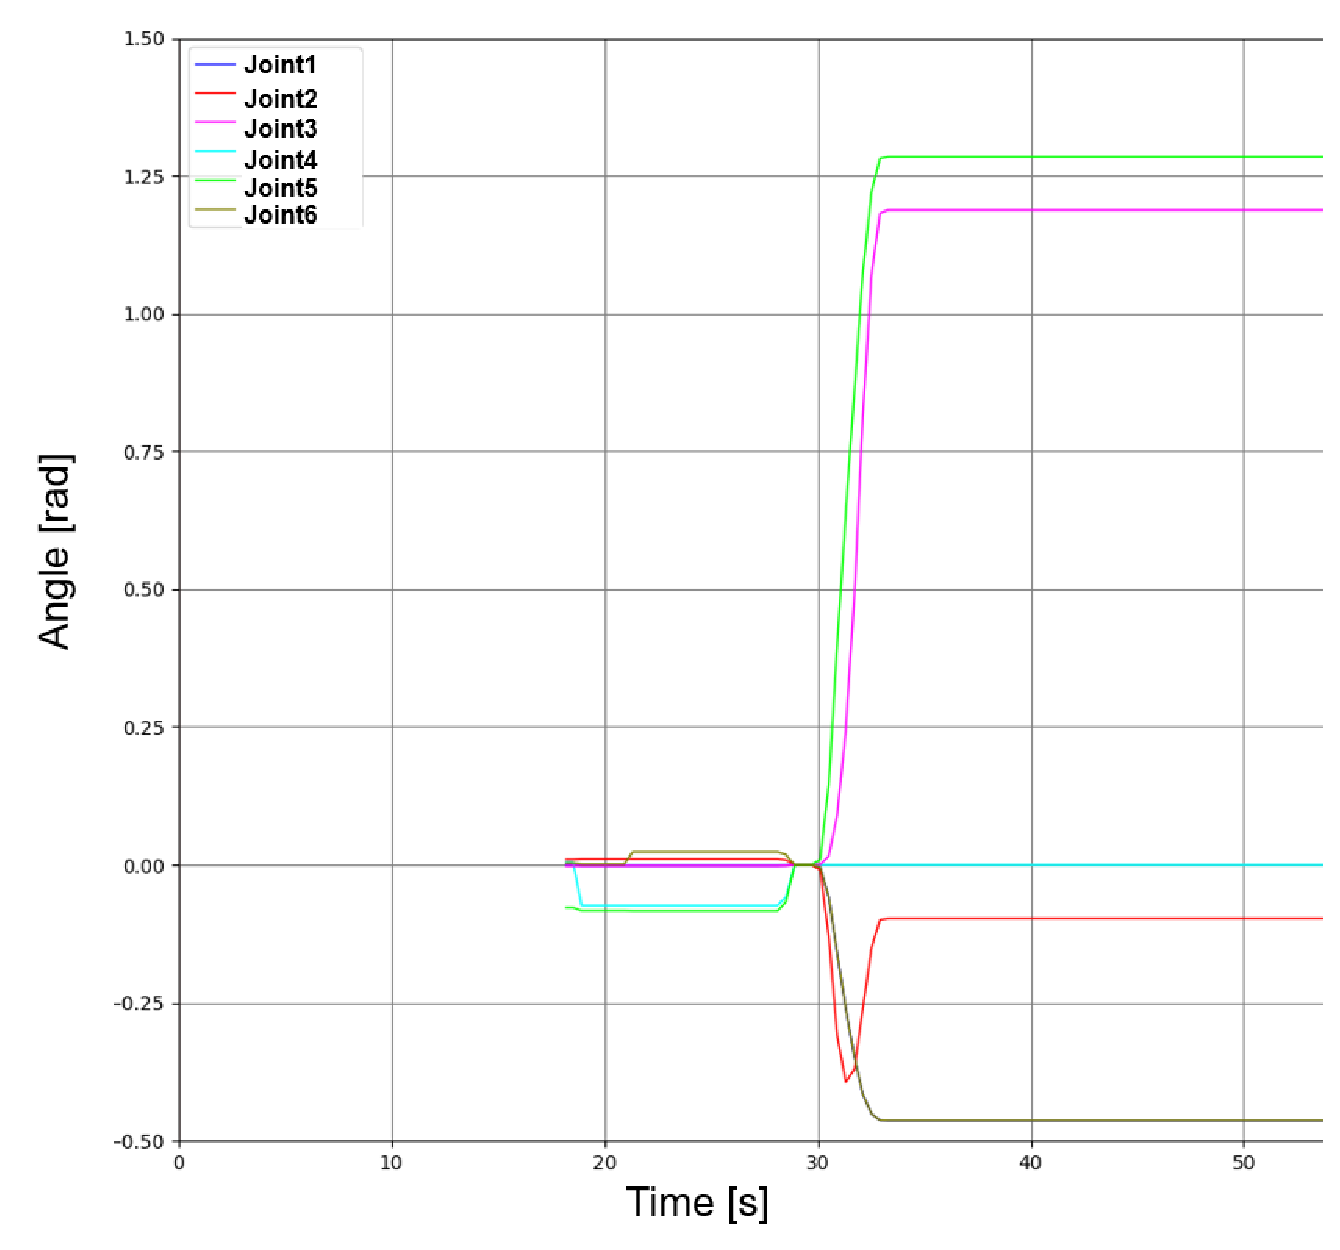
\includegraphics[height=90mm]{expt_8_joint_states.eps}
     \caption{物理モデル実験のLite6の各関節の角度変化}
     \label{fig:f2}
\end{figure}

\begin{table}[htb]
	\centering
	\caption{Lite6の物理モデルの目標手先座標到達後の各関節の角度}
	\begin{tabular}{lcrc} \hline
	Joint Name& Value     \\ \hline \hline
	Joint1    & $-26.5657^\circ$ \\
	Joint2    & $-95.5362^\circ$ \\
	Joint3    & $-21.9537^\circ$ \\
	Joint4    & $0.00532082^\circ$ \\
	Joint5    & $73.5847^\circ$ \\
    Joint6    & $-26.5649^\circ$ \\ \hline
	\end{tabular}
\end{table}

\begin{figure}[htbt]
    \centering
     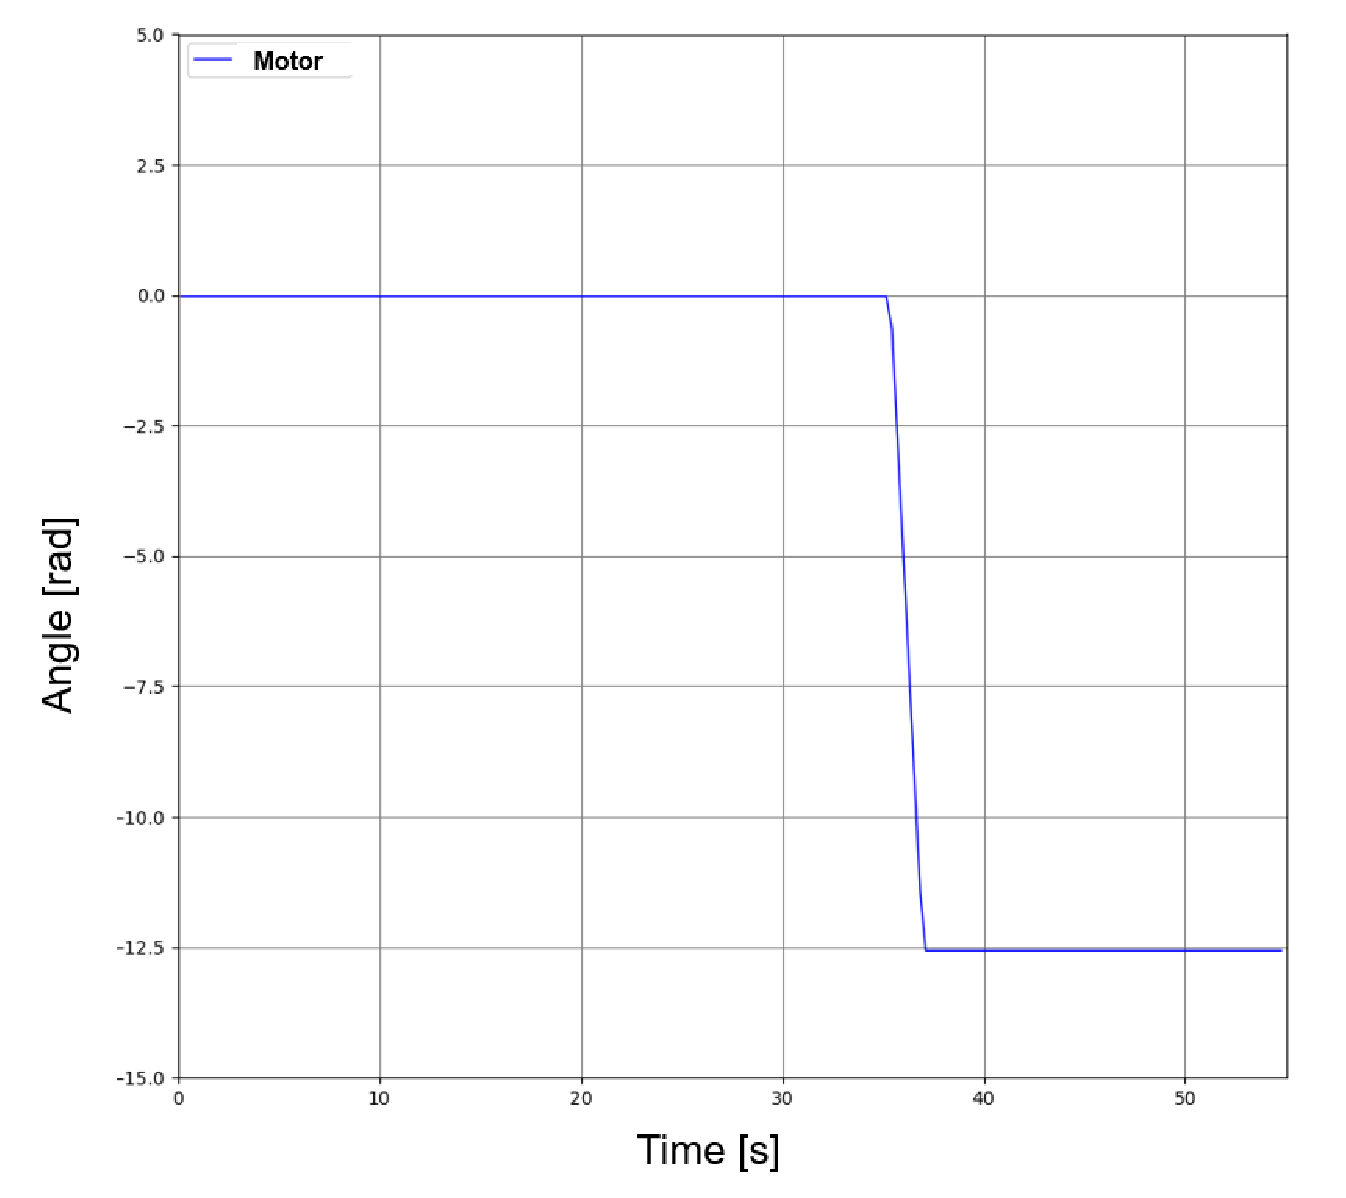
\includegraphics[height=90mm]{expt_8_dyna.eps}
     \caption{切り紙グリッパーの物理モデル実験の角度変化}
     \label{fig:f2}
\end{figure}

\subsection{デジタルモデルの実験結果}
次に,デジタルモデルの実験結果を以下に示す.
図3.7から,0sから5sにかけて手先が目標の手先座標に移動していることがわかり,このとき各関節の角度は図3.8に示すように変化した.変化後の各関節の角度を表3.2にまとめる.
また,Lite6の基準座標系から手先座標系までの同次変換行列に表3.2の角度を代入して計算すると実際の手先座標は(0.177684, -0.0850857, 0.268569) mになった.\\
 そして,図3.7から7sから9sにかけて切り紙グリッパーが閉じていることがわかる.このとき切り紙グリッパーのデジタルモデルに追加した指先距離測定用ジョイントのY座標の変化は図3.9のようになった.
図3.9では,指先距離測定用ジョイントのY座標が約22 sから急激に上がっているが,これが目標手先座標に移動したときの変化であり,切り紙グリッパーを閉じたときの変化は約28 sから約30 sである.
したがって,指先距離測定用ジョイントのY座標が切り紙グリッパーが初期位置で開いた状態から完全に閉じるまでに移動した距離は0.0250162 mになった.


\begin{figure}[htbt]
    \centering
     \includegraphics[height=90mm]{simmove.eps}
     \caption{デジタルモデル実験の結果}
     \label{fig:f2}
\end{figure}

\begin{figure}[htbt]
    \centering
     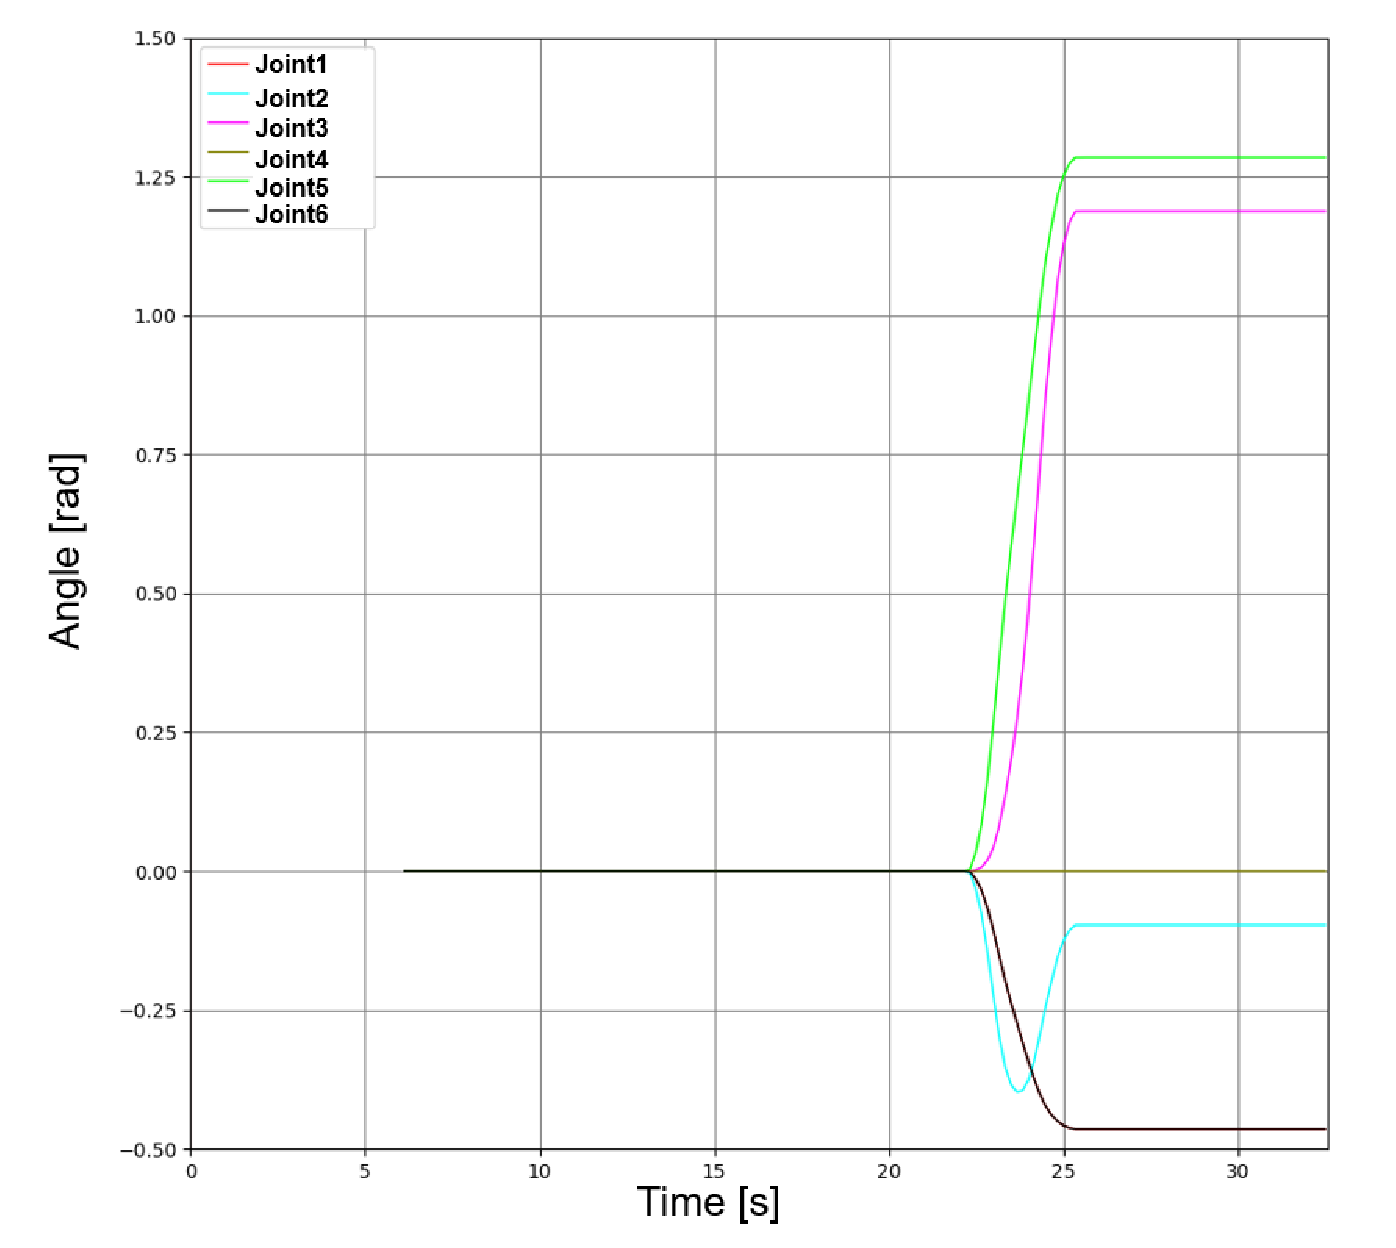
\includegraphics[height=90mm]{expt_8_sim_joint_states.eps}
     \caption{デジタルモデル実験のLite6の各関節の角度変化}
     \label{fig:f2}
\end{figure}

\begin{table}[htb]
	\centering
	\caption{Lite6のデジタルモデルの目標手先座標到達後の各関節の角度}
	\begin{tabular}{lcrc} \hline
	Joint Name& Value     \\ \hline \hline
	Joint1    & $-26.5656^\circ$ \\
	Joint2    & $-95.5366^\circ$ \\
	Joint3    & $-21.9535^\circ$ \\
	Joint4    & $0.00721438^\circ$ \\
	Joint5    & $73.5848^\circ$ \\
    Joint6    & $-26.5648^\circ$ \\ \hline
	\end{tabular}
\end{table}


\begin{figure}[htbt]
	\centering
	 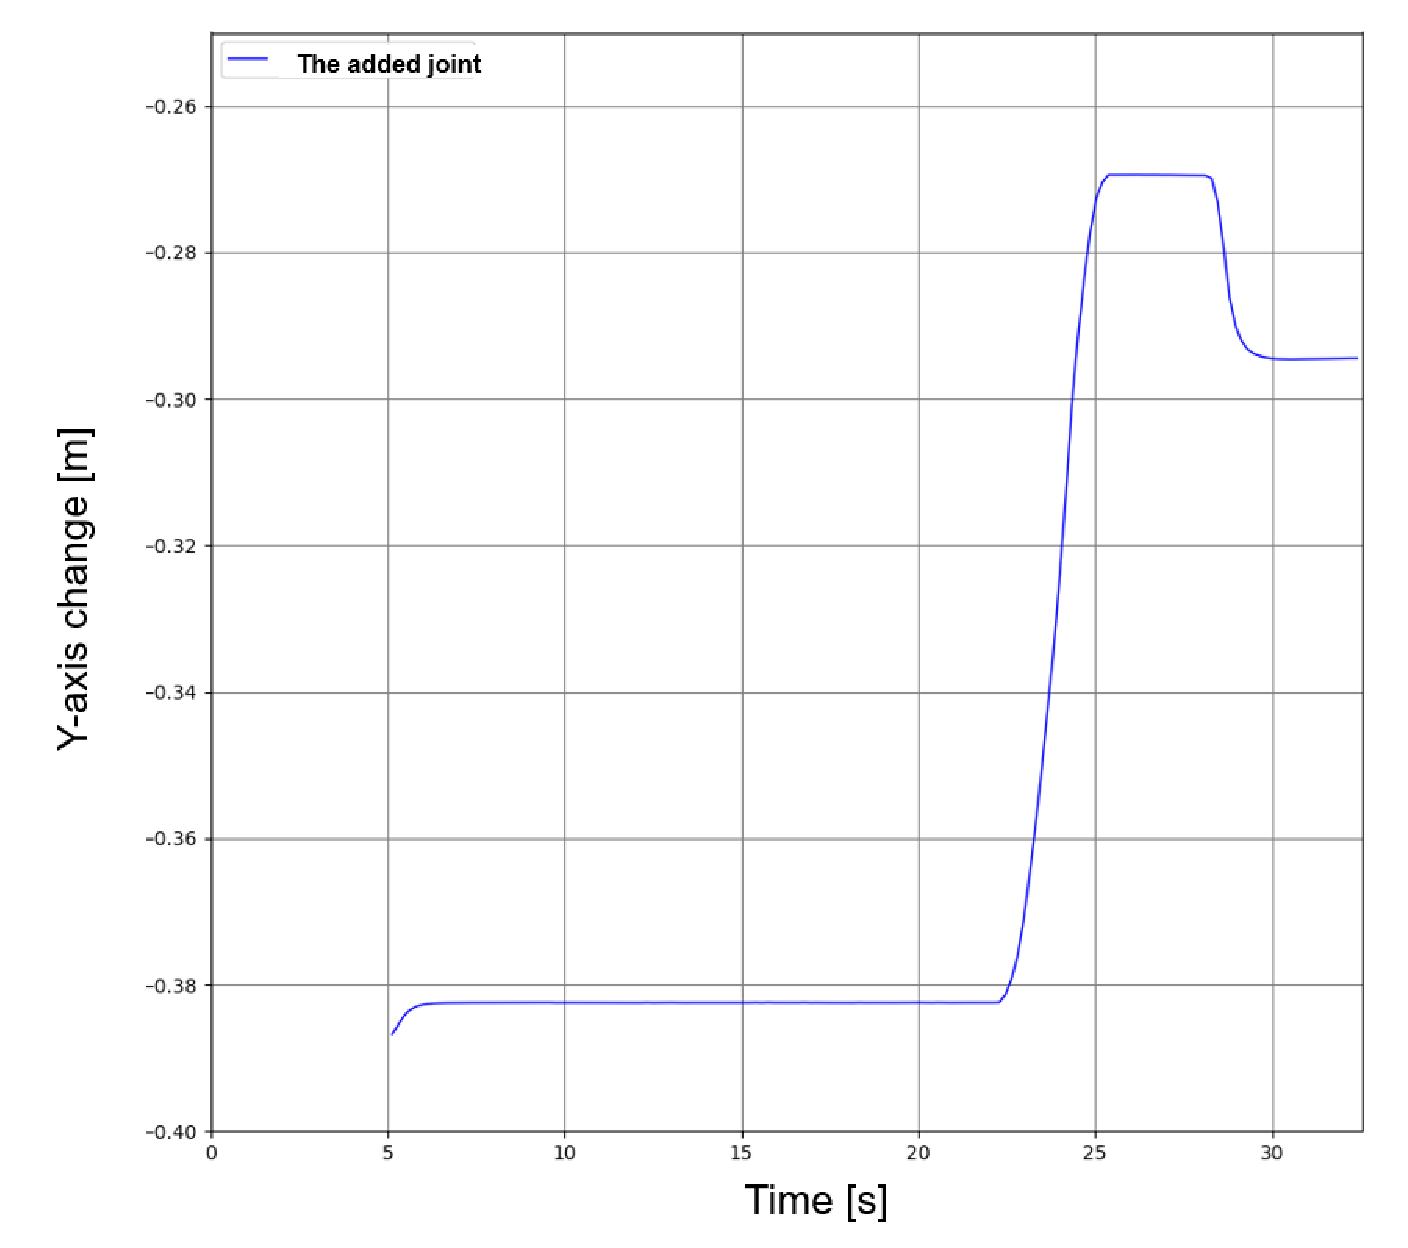
\includegraphics[height=90mm]{measure_joint_evi.eps}
	 \caption{切り紙グリッパーのデジタルモデルに追加した指先距離測定用ジョイントのY座標の変化}
	 \label{fig:f2}
\end{figure}

\section{考察}
本節では,前節でまとめた物理モデルとデジタルモデルの実験結果に基づいて考察を述べる.\\
 まず,ロボットアームの手先位置のデジタルツインについて考察を述べる.
図3.4と図3.7を比較すると,目標手先座標へ到達するまでにかかった時間は物理モデルとデジタルモデルの間でほとんど差は見られなかった.\\
 Lite6の基準座標系から手先座標系までの同次変換行列とrosbagコマンドで収集した目標手先座標到達後の各関節の角度で求めた,
物理モデルの現実空間での手先座標とデジタルモデルのGazebo空間での手先座標はそれぞれ(0.177674, -0.0850884, 0.268573) m,(0.177684, -0.0850857, 0.268569) mであり物理モデルとデジタルモデルの間でほとんど差は見られなかった.
しかし,目標手先座標(0.20750, -0.10000, 0.25875) mから物理モデルは(0.029816, -0.014912, -0.0098230) m,デジタルモデルは(0.029816, -0.0149143, -0.009819) mの差があり,特にX座標の差が大きい.
この原因として切り紙グリッパーの重心がLite6の第6リンクの中心よりもX軸の前方にあり,その重さの前方への偏りによって手先が前方へ行き過ぎないように各関節のトルクに抑制がかかっている可能性が考えられる.
この問題は各関節のPIDゲインを調整することや切り紙グリッパーを重心を考慮して再設計することで解決できると考えられる.\\
 以上より,ロボットアームの手先位置のデジタルツインは,実行時間については差が少なくデジタルツインができており,手先位置についても座標軸によって差があるものの数センチメートルの範囲に抑えられているためデジタルツインができたと言える.

次に,切り紙グリッパーの指先距離のデジタルツインについて考察を述べる.
図3.4と図3.7を比較すると,切り紙グリッパー初期位置で開いた状態から完全に閉じるまでにかかった時間は物理モデルとデジタルモデルの間でほとんど差は見られなかった.
そして,切り紙グリッパーのグリッパーの中心から指先までの距離は実測値で,閉じたとき0 mm,開いたとき27 mmであった.
指先距離測定用ジョイントのY座標が切り紙グリッパーが初期位置で開いた状態から完全に閉じるまでの変化量は0.0250162 mであり,単位を合わせると約25 mmであった.\\
 以上より,切り紙グリッパーの指先距離のデジタルツインは,実行時間については差が少なくデジタルツインができており,指先距離についても数ミリメートルの差はあるもののデジタルツインができたと言える.